\chapter{Metode}
\textit{I dette kapitel beskrives formålet med udviklingen af beslutningsstøttesystem til risikovurdering af lægemidler, hvordan data er indsamlet samt hvilken proces der er gennemgået i forhold til udvikling for algoritme til risikovurdering som beslutningsstøtte.}

\section{Formål}
På nuværende tidspunkt vurderes kompleksiteten af implementering af lægemiddelskift af ATC-ansvarlige ud fra tidligere erfaringer og viden indsamlet via bl.a. pro.medicin. Flere faktorer vægtes ved vurderingen, hvilket gør denne proces meget personafhængig og stiller visse krav til den ATC-ansvarliges viden og erfaring inden for området. Vurderingen der foretages har betydning for implementeringen af lægemiddelskiftet i klinikken og det er derfor vigtigt at den rette vurdering foretages i forhold til at undgå medicineringsfejl som f.eks. forveksling af navnet på lægemidlet grundet ændringer af ved lægemiddelskift. 
For at imødekomme disse problemstillinger ønskes det at udvikle et beslutningsstøttesystem til den ATC-ansvarlige som foretager risikovurderingen af lægemiddelskift med henblik på at synliggøre de ændringer som sker ved et eventuelt lægemiddelskift, hvormed den ATC-ansvarlige har et bedre beslutningsgrundlag.

\section{Dataindsamling}
Data er indsamlet af Amgros og Sygehusapoteket Region Nordjylland (SRN) og omhandler lægemiddelskift i år 2018. Data fra Amgros omhandler oplysninger om lægemiddelskiftet foretaget fra år 2017 til 2018. Yderligere har Amgros udarbejdet et dokument over risikolægemidler. Risikolægemidler er lægemidler som er særligt risikofyldte hvis disse ender i restordre, da erstatninger er svære at finde samt risikoen for fejl øges ved erstatning. Data fra SRN omhandler de udbud af lægemidler Amgros foretog inden et eventuelt kontraktskift for år 2018. 
%Udover dette har SRN ligeledes indsamlet de problemstillinger der har været vedrørende Amgrosskift siden år 2012.  


\section{Udviklingsproces}
Udviklingen af et beslutningsstøttesystem bygger på forskellige processer herunder valg af features, præprocessering, design, implementering og test. Udviklingstrinene fremgår af Figur \ref{fig:metode}.

\begin{figure}[H]\centering	\includegraphics[width=1\textwidth]{billeder/udviklingstrin.png} 
	\caption{Udviklingstrin for beslutningsstøttesystem}
	\label{fig:metode}  
\end{figure}
\vspace{-0.5cm}

Af Figur \ref{fig:metode} illustreres de forskellige processer som der foretages ved udviklingen af beslutningsstøttesystemet. Udvælgelsen af features danner grundlag for de inputs som skalvægtes i forhold til beslutningen. Da data ikke er homogen ønskes det at foretage præprocessering på data for at gøre det sammenligneligt. Design bygger på design af algoritmen, denne verificeres i løbet af processen for at opnå det bedst mulige design. Efter designfasen implementeres systemet, hvorefter dette testes. I testfasen valideres hvorvidt systemet performer efter formålet, hvis dette ikke er tilfældet kan der vendes tilbage til de fortgående udviklingstrin i forhold til at omformulere i forhold til præprocessing, redesigne i designfasen eller tilpasse i implementeringsfasen. 



%Første trin omhandler identificering af problemer som systemet skal løse, herunder data som systemet skal arbejde på og tilgængelige ressourcer~\citep{Ligeza2006}. Det andet trin er omhandler identificering af nøglekoncepter samt relationer mellem disse som f.eks. typer af data, informationsstrøm og underliggende stukturer. Tredje trin involverer forståelse, beskrivelse og formalisering af problemet og hvordan løsninger findes. Denne proces bør omfatte verificering af systemet. Det fjerde trin har til formål at implementere den formaliseret viden i et program. Det sidste trin omfatter test ved validering af regler og implementeringen.~\citep{Ligeza2006}


\chapter{Systemanalyse}
\section{Valg af features}
Features er udvalgt på baggrund af retningslinjer for den ATC-ansvarlige, som fremgår af Appendiks~\ref{cha:AppD}, og litteratur som beskriver ændringer i forskellige faktorer som har ledt til medicineringsfejl i klinikken som følge af lægemiddelskift. Derudover er information omkring risikolægemidler og komplekse ATC-koder anvendt som er indsamlet af Amgros eller er dokumenteret i forbindelse med Amgrosudbud af SRN.
Features og begrundelse for valg af features fremgår af Tabel \ref{table:features}.

\begin{longtable}{p{3.5cm}| p{10.5cm}}
	\caption{Valg af features}
	\label{table:features} \\
\cellcolor[HTML]{C0C0C0} {\textbf{Feature}} & \cellcolor[HTML]{C0C0C0} {\textbf{Begrundelse}}  \\ \hline
\textbf{Navn} &  Forveksling ved ændringer i navn på lægemidler er en af de hyppigste årsager til medicineringsfejl jævnfør afsnit \ref{sec:ProblemLaeg} [X]. Forvirring over ikke at kunne finde lægemidlet fordi navnet har ændret sig \\  \hline 
\textbf{Lignende navne} &  Forveksling ved ændringer i navn på lægemidler er en af de hyppigste årsager til medicineringsfejl jævnfør afsnit \ref{sec:ProblemLaeg}. [X] Disse forekommer grundet allerede eksisterende lægemiddel jævnfør afsnit \ref{sec:ProblemLaeg}. [X]. \\  \hline 
\textbf{Dispenseringsform} &  FIND BEGRUNDELSE FOR DETTE  \\ \hline 
\textbf{Styrke} &  Forkert dosis er dokumenteret se kilde 18,19,20 og 21  \\ \hline
\textbf{Risikolægemidler} & Disse lægemidler kan være problematiske, hvis de ender i restordre, altså at lægemidlet ikke kan leveres og det derfor er nødvendigt at finde et erstatningslægemiddel. Disse lægemidler bør være på lager, da det er svært at finde erstatninger for disse samt risikoen for fejl øges ved erstatning. Beskrevet i Appendiks ~\ref{cha:AppD}[FIND KILDE, eller indsæt i appendiks]  \\ \hline 
\textbf{ATC-koder} &  Der er nogle ATC-koder som er mere komplekse end andre. Dette er f.eks. på områder som indgår i produktionen på Sygehusapoteket Region Nordjylland og væsker, hvor en ændring i leverandør typisk vil forårsage ændringer af device, hvilket kan skabe problemer i klinikken. [KILDE] \\ \hline 
\textbf{Medicinråd} & Nogle lægemidler omhandler medicinrådets behandlingsvejledninger. Disse lægemidler omfatter enkelte hospitalsafdelinger og kræver et tæt samarbejde med disse. Det ønskes ligeledes at lægemidlet implementeres hurtigt, da det er muligt at opnå store besparelser. [KILDE + APPENDIKS]\\ \hline 
\textbf{Pris} &  Pris er vigtigt i forhold til at opnå besparelser. Det skal ligeledes vægtes om det kan betale sig at skifte et lægemiddel med mindre besparelse, da udskiftningen kan få store betydninger for klinikken i forhold til arbejdsgangen og i værste tilfælde medføre patientsikkerhedsmæssige konsekvenser. [KILDE, AMGROS] \textcolor{blue}{Det er endnu ikke besluttet, hvordan denne faktor skal indgå i algoritmen.} \\ \hline
    \end{longtable}

\section{Præprocessering}
Data er manuelt indskrevet og indeholder tekst og er derfor ikke sammenligneligt, hvorfor data er præprocesseret før anvendelsen. Da det er forskelligt om data er skrevet med majuskel eller minuskel er det valgt at ændre alt data til minuskel. Noget data er skrevet med forkortelser hvorfor det er valgt at fjerne forkortelser og udskrive ordene med henblik på at gøre data generaliserbar. 

Der er derudover lavet antagelser for navn og dispenseringformer for lægemidler. Det er valgt kun at kigge på præfiks for alle lægemidler, hvorfor præfiks er fjernet fra alle lægemidler. Der er dog nogle lægemidler  hvor ændring i præfiks betyder ændringer i styrke og dispenseringsform. Det er dog antaget at denne tages højde for i sammenligning af ændringer i styrke og dispenseringsform. Ligledes antages det for dispenseringsformer som tabletter at disse er ens hvis dispenseringsform er en af følgende; filmovertrukne, overtrukne eller  tabelletter. \textcolor{blue}{Om der er tale om væske og opløselig væske. Tilføj også for styrke når dette er undersøgt. Derudover bliver der også fjernet forlængelser som det første - skriv dette til}

\textcolor{red}{Ved ikke om det giver mening at gøre dette mere konkret her ved at komme med eksempler eller om jeg godt kan vente med dette til implementering og vise det der.Synes at dette vil give mere mening.}

\section{Design}
\textcolor{red}{Tænker at dette afsnit skal være et flowdiagram over algoritmen som det billede jeg har sat ind på Figur  \ref{fig:algoritme}.} 
\begin{figure}[H]\centering	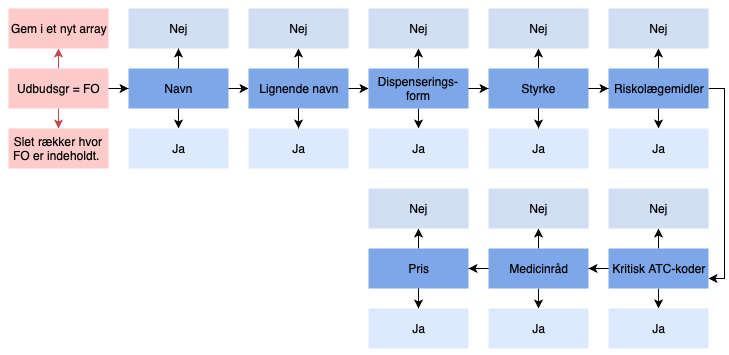
\includegraphics[width=1\textwidth]{billeder/algoritme.png} 
	\caption{Flowchart af algoritme}
	\label{fig:algoritme}  
\end{figure}
\vspace{-0.5cm}


\chapter{Implementering}

\section{Program}
Det er valgt at implementere i NetBeans som er et integreret udviklingsmiljø (IDE) til Java. Der er tilføjet biblioteker som JExcelApi og Apache POI til håndtering af Microsoft dokumenter herunder excel.

\section{Præprocessering}
\textcolor{red}{Jeg tænker at dette kan repræsenteres som pseudo code eller tabel eller screendumps af kode.} 

\section{Algoritme}
\textcolor{red}{Tænker at dette afsnit skal være et pseudo code over algoritmen som det billede jeg har sat ind på Figur  \ref{fig:pseudo}. Denne figur er kun udkast og er blot få en idé af hvordan jeg har tænkt mig at implementere algoritmen. Jeg tænker at det output der skal komme ud af algoritmen er tekst som skriver hvad der er ændret. Ved ikke om der kunne  være en fordel i at dele dette op på en måde? Men tænker bare at selve koden er det samme for meget af det.}
\begin{figure}[H]\centering	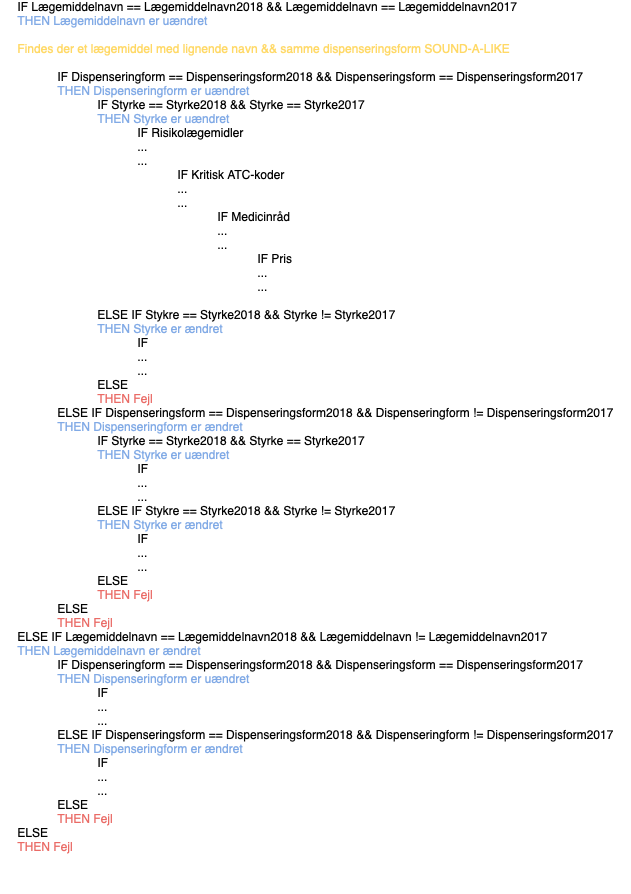
\includegraphics[width=1\textwidth]{billeder/Pseudo.png} 
	\caption{Pseudo code}
	\label{fig:pseudo}  
\end{figure}
\vspace{-0.5cm}


\chapter{Test}
\textcolor{red}{Tænker at teste noget i forhold til falsk/positive. Hvor mange gang gør algoritmen det den skal?}

